\documentclass[11pt, a4paper, titlepage]{article}
\usepackage[left=1.5cm,text={18cm, 25cm},top=2.5cm]{geometry}
\usepackage[utf8]{inputenc}
\usepackage[czech]{babel}
\usepackage{hyperref}
\usepackage{amsmath}
\usepackage{graphicx}
\usepackage{wrapfig}
\usepackage{caption}
\usepackage{subcaption} % add sub figures
\usepackage{amsfonts}

% \usepackage{subfig}
% \usepackage{color}
% \usepackage{times}
% \usepackage[bf]{caption}
% \usepackage{hyperref}
% \usepackage[all]{hypcap}
% \usepackage{graphicx}
% \usepackage{url}
% \usepackage[all]{hypcap}
% \hypersetup{colorlinks=false, linkbordercolor=1 1~1, citebordercolor=1 1~1}
% \usepackage[right]{lineno}
% \usepackage{listings}
% \renewcommand\linenumberfont{\normalfont\tiny\color{blue}}

\iflanguage{english}{
    \renewcommand{\uv}[1]{``#1''}
}


%--------------------------------------------------------------------------------


\begin{document}
\begin{titlepage}
    \begin{center}
        \textsc{\LARGE Fakulta informačních technologií}\\
        \vspace{0.1 cm}
        \textsc{\LARGE Vysoké učení technické v~Brně}\\
        \vspace{\stretch{0.39}}
        {\Huge MUL -- Multimédia}\\
        \vspace{\stretch{0.01}}
        {\huge Aplikace pro zpracování obrázků a~videí}
        \vspace{\stretch{0.62}}
    \end{center}
    \begin{center}
    \Large
    Petr Fusek \\
    xfusek08@stud.fit.vutbr.cz \\
    \today
    \end{center}
\end{titlepage}


\section{Zadání}
Implementujte aplikaci, která bude umožňovat zpracování obrázků (ostření, hrany, úprava barevnosti).
Kromě kvalitního GUI též implementujte schopnosti aplikace pro práci s~videosekvencemi - spouštění, zjištění kodeku, výběr/vložení úseku apod.

\section{Zvolené Technologie}
Pro implementaci multiplatformní aplikace s~grafickým uživatelským rozhranním byl zvolen programovací jazyk \texttt{Rust}\footnote{\url{https://www.rust-lang.org/}}, který v~poslední době nabývá na popularitě především v~rámci open-source komunity a~klade si za cíl být systémovým programovacím jazykem nové generace.
Jeho výhody jsou ve vysoké úrovni abstrakce a~formálnosti, která zaručuje bezpečnou práci s~pamětí, bez obětování výkonu během jeho běhu (neobsahuje interpret ani \emph{garbage collector}) a~tím dosahuje výkonu srovnatelného s~\texttt{C++}.

Pro implementaci grafického uživatelské rozhraní je použita knihovna \texttt{egui}\footnote{\url{https://github.com/emilk/egui}}, která alternativou populárního \texttt{Dear ImGui} (\texttt{C/C++}) pro implementovaná v~Rustu a~na pozadí používá grafické API \texttt{OpenGL}\footnote{\url{https://www.opengl.org/}}.
Díky těmto technologiím lze aplikaci přeložit téměř pro všechny platformy podporující \texttt{OpenGL}.

\subsection{Seznam použitých knihoven}
Toto je kompletní seznam knihoven a~ke kterému účelu byly použity během implementace.
\begin{itemize}
    \item {
        \texttt{egui} - \emph{immediate mode} grafické uživatelské rozhraní.\\
        {\small\url{https://github.com/emilk/egui}}
    }
    \item {
        \texttt{file-format} - Detekce správného formátu vstupního souboru.\\
        {\small\url{https://github.com/mmalecot/file-format}}
    }
    \item {
        \texttt{rfd} - Multiplatformní dialog pro výběr vstupního souboru.\\
        {\small\url{https://github.com/PolyMeilex/rfd}}
    }
    \item {
        \texttt{indoc} - Vylepšení nativních maker ve zdrojovém kódu.\\
        {\small\url{https://github.com/dtolnay/indoc}}
    }
    \item {
        \texttt{image} - Knihovna pro zpracování obrázků.\\
        {\small\url{https://github.com/image-rs/image}}
    }
    \item {
        \texttt{cgmath} - Abstraktní matematická knihovna obsahující vektorový a~maticový počet.\\
        {\small\url{https://github.com/rustgd/cgmath}}
    }
\end{itemize}

\section{Implementace}
V rámci projektu byl implementován jednoduchý editor, umožňuje a~aplikovat různé barevné filtrovací operace/transformace pro obrázky ve formátu \texttt{jpeg}.

\subsection{Popis aplikace}

Rozložení grafického rozhraní aplikace ukazuje obrázek \ref{fig:screenshot}.
Aplikace funguje tak, že po spuštění se objeví uvítací obrazovka, která vyzve uživatele aby vybral obrázek ze svého počítače.
Poté mu je umožněno aplikovat sérii filtrů, jejichž efekty jsou viditelné v~reálném čase.
Filtry jsou aplikovány v~sérii za sebou v~pořadí shora dolů, jak jsou vykresleny.
Při stisknutí mezerníku se zobrazí originální obrázek bez úprav.
Nahází se zde tlačítko \uv{Open}, které umožní změnit právě editovaný obrázek za jiný z~počítače.
Po dokončení úprav je možné soubor uložit pomocí tlačítka \uv{Save}.
Na spodní liště jsou vidět informace o~právě editovaném obrázku.

\begin{figure}
    \centering
    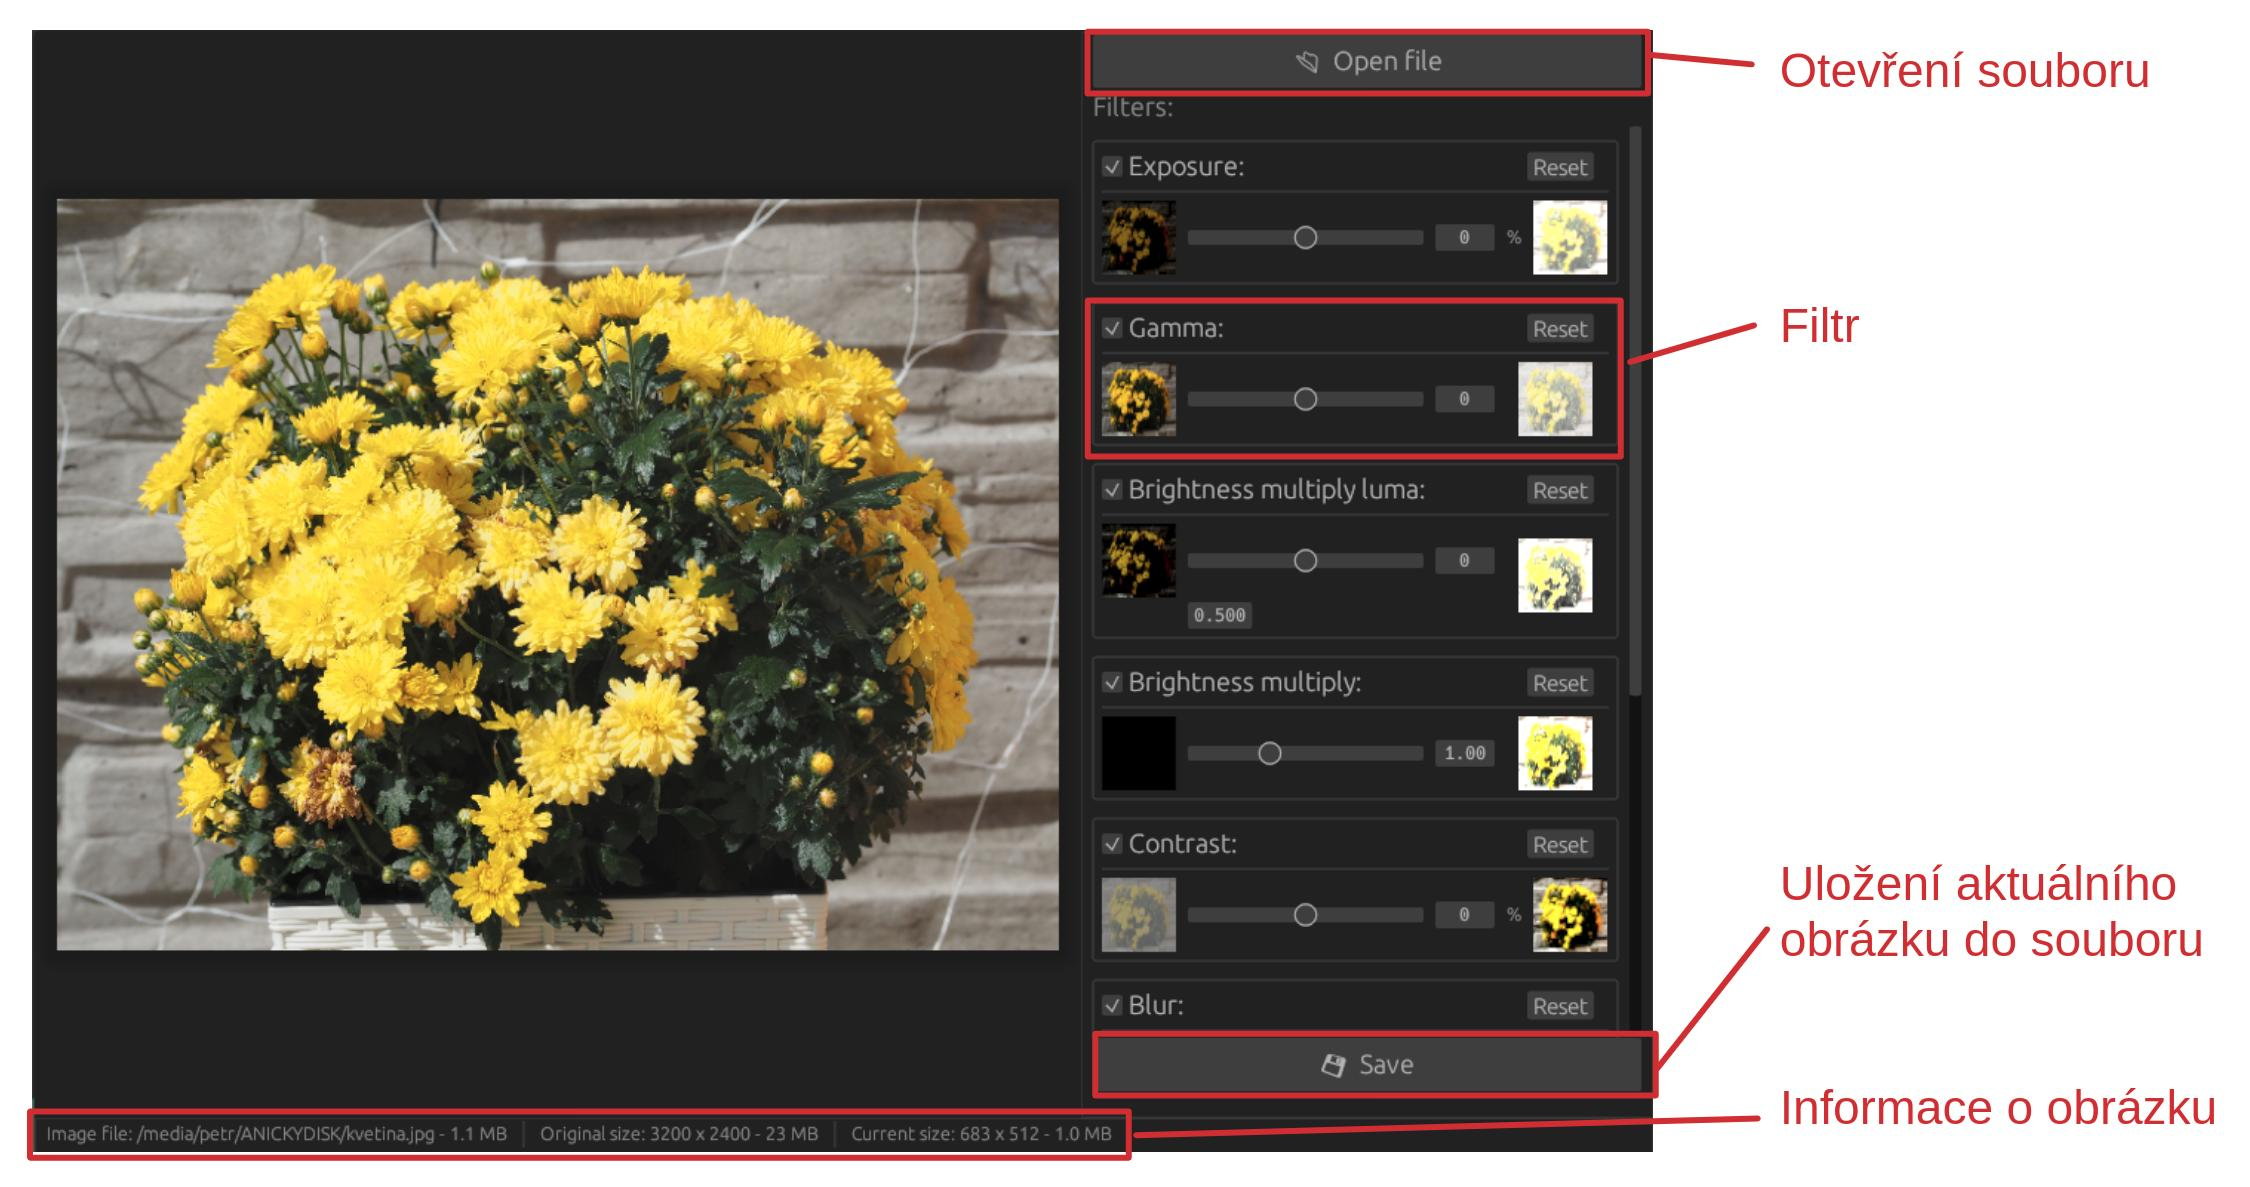
\includegraphics[width=0.9\textwidth]{screenshot.jpg}
    \caption{Snímek hlavní obrazovky editoru}
    \label{fig:screenshot}
\end{figure}

\subsection{Popis implementovaných filtrů}

\subsubsection{Expozice}
Nejjednodušším filtrem je expozice, která je součástí každého editoru.
její implementace spočívá v~přičtení konstantní hodnoty ke všem subpixelům.
$$P' = \delta + P$$
Na obrázku \ref{fig:exposure} je vidět přičtení záporné hodnoty pro ztmavení a~kladné pro zesvětlení.
\begin{figure}[h]
    \centering
    \begin{subfigure}[t]{0.25\textwidth}
        \vskip 0pt
        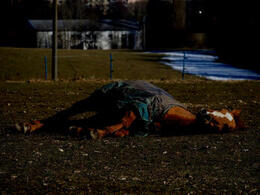
\includegraphics[width=1.0\textwidth]{horse_exposure_minus.jpg}
        \caption{Záporná expozice - ztmavení obrázku}
    \end{subfigure}
    \hspace{1cm}
    \begin{subfigure}[t]{0.25\textwidth}
        \vskip 0pt
        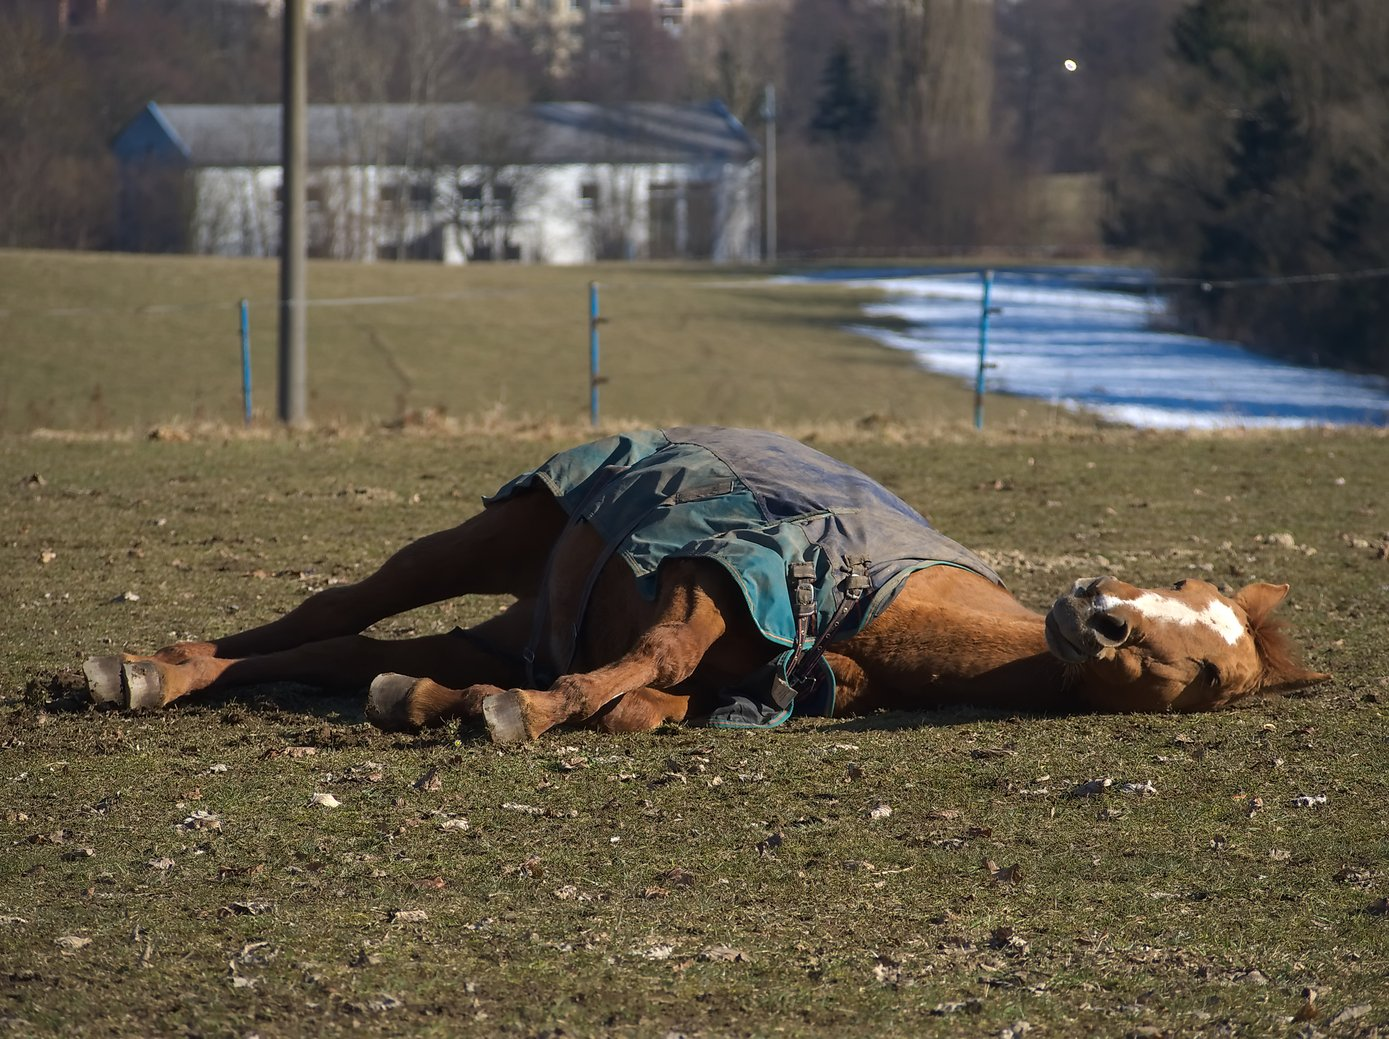
\includegraphics[width=1.0\textwidth]{horse_original.jpg}
        \caption{Původní obrázek}
    \end{subfigure}
    \hspace{1cm}
    \begin{subfigure}[t]{0.25\textwidth}
        \vskip 0pt
        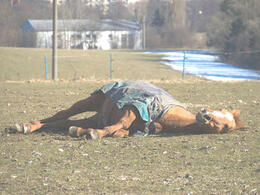
\includegraphics[width=1.0\textwidth]{horse_exposure_plus.jpg}
        \caption{Kladná expozice - zesvětlení obrázku}
    \end{subfigure}
    \caption{Výsledky operace \uv{Expozice}}
    \label{fig:exposure}
\end{figure}
Zde je vidět, že efekt není příliš šetrný a~způsobuje bílou mlhu a~nezachovává stíny.

\subsubsection{Gamma}
Gamma korekce je nelineární transformace pracující s~jasovou složkou obrázku.
Počítá se umocněním jasu na hodnotu $\gamma \leq 0$ \cite{wiki:Gamma_correction}.
$$V_{out}=V_{in}^\gamma$$
Pokud $\gamma < 1.0$ tmavší pixely budou zesvětleny a~čím více pixel světlejší je, tím méně bude ovlivněn.
Při $\gamma > 1.0$ budou hodnoty tmavších pixelů zredukovány a~zvýší se tak kontrast světlé vůči tmavé.
Výsledek této operace je vidět na obrázku \ref{fig:gamma}.
\begin{figure}[h]
    \centering
    \begin{subfigure}[t]{0.25\textwidth}
        \vskip 0pt
        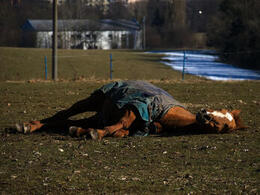
\includegraphics[width=1.0\textwidth]{horse_gamma_minus.jpg}
        \caption{Obrázek pro $\gamma = 0.5$}
    \end{subfigure}
    \hspace{1cm}
    \begin{subfigure}[t]{0.25\textwidth}
        \vskip 0pt
        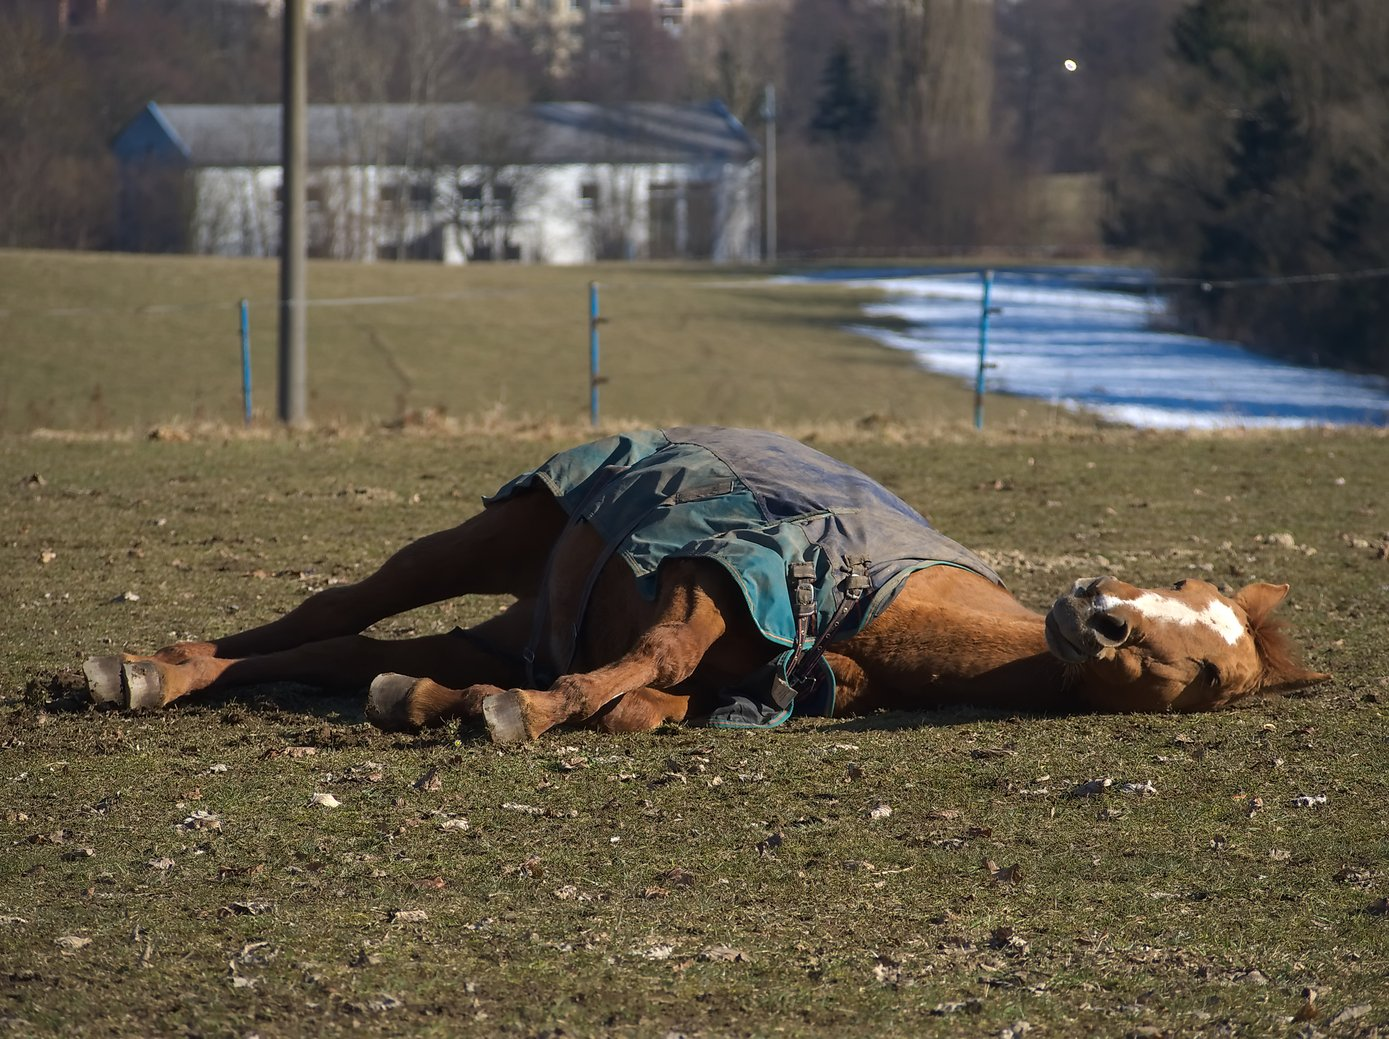
\includegraphics[width=1.0\textwidth]{horse_original.jpg}
        \caption{Původní obrázek ($\gamma = 1$)}
    \end{subfigure}
    \hspace{1cm}
    \begin{subfigure}[t]{0.25\textwidth}
        \vskip 0pt
        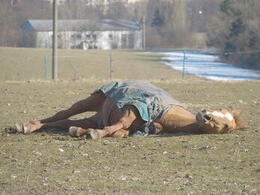
\includegraphics[width=1.0\textwidth]{horse_gamma_plus.jpg}
        \caption{Obrázek pro $\gamma = 1.5$}
    \end{subfigure}
    \caption{Výsledky operace \uv{Gamma}}
    \label{fig:gamma}
\end{figure}
Oproti jednoduché expozici bílá mlha není tak nápadná a~ztmavení se jeví více vyrovnaným dojmem.

\subsubsection{Kontrast}
Úprava kontrastu znamená, že měníme relativní rozdíl barvy a~jasu pixelu oproti středí hodnotě celého obrázku \cite{wiki:Contrast_vision}.
Současná implementace je v~tomto případě záležitostí použité knihovny \texttt{image}.
Výsledek je vidět na obrázku \ref{fig:contrast};
\begin{figure}[h]
    \centering
    \begin{subfigure}[t]{0.25\textwidth}
        \vskip 0pt
        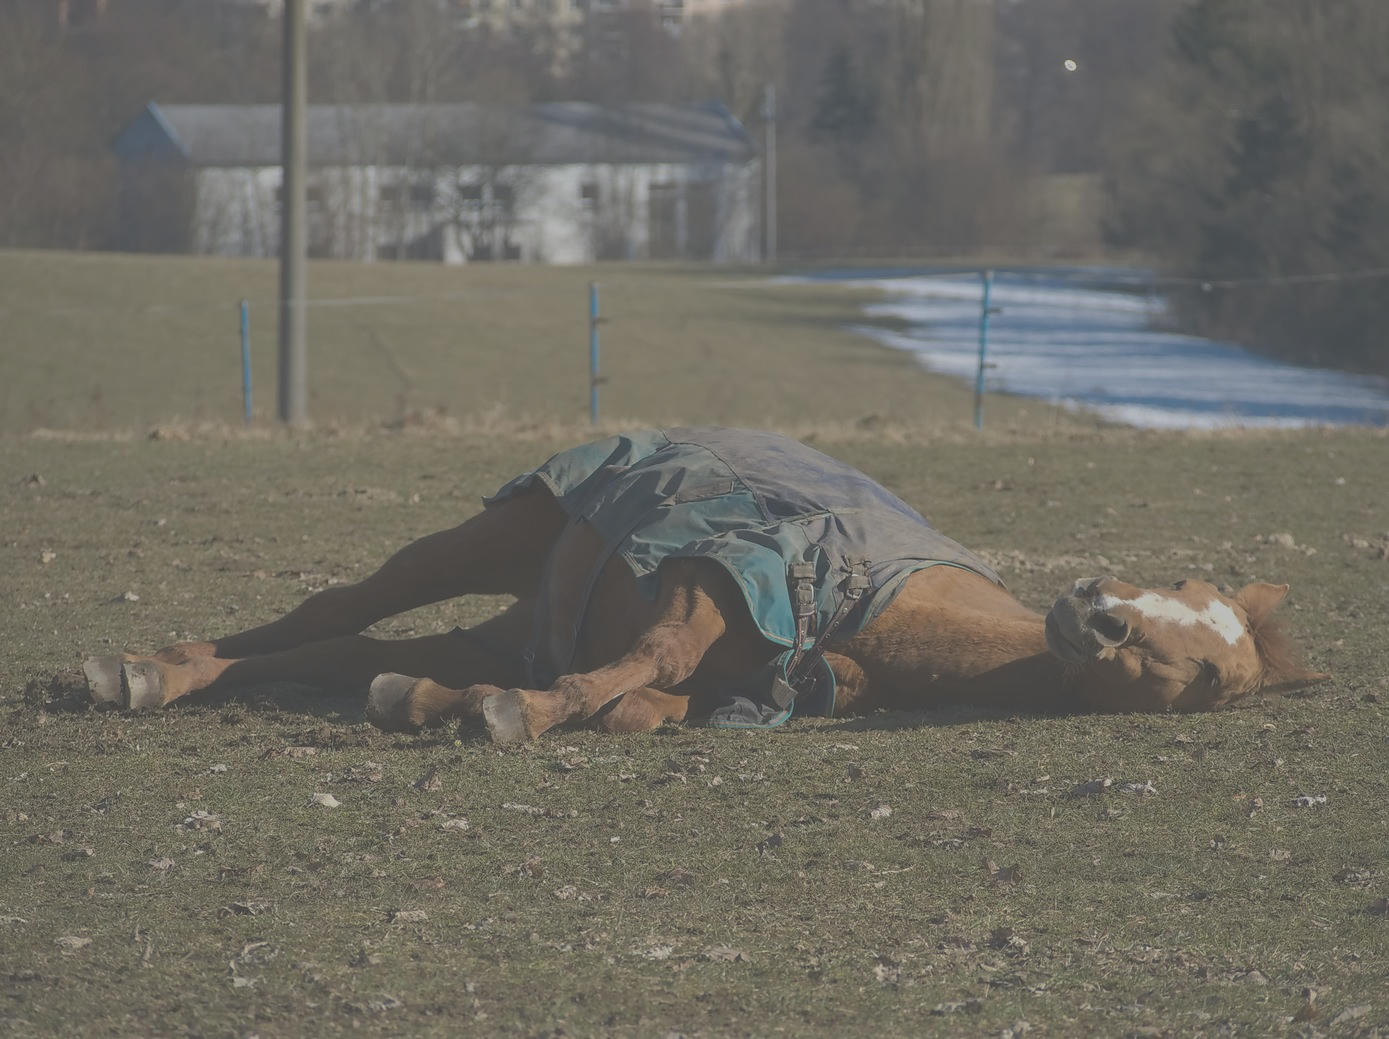
\includegraphics[width=1.0\textwidth]{horse_contrast_minus.jpg}
        \caption{Snížený o~50\%}
    \end{subfigure}
    \hspace{1cm}
    \begin{subfigure}[t]{0.25\textwidth}
        \vskip 0pt
        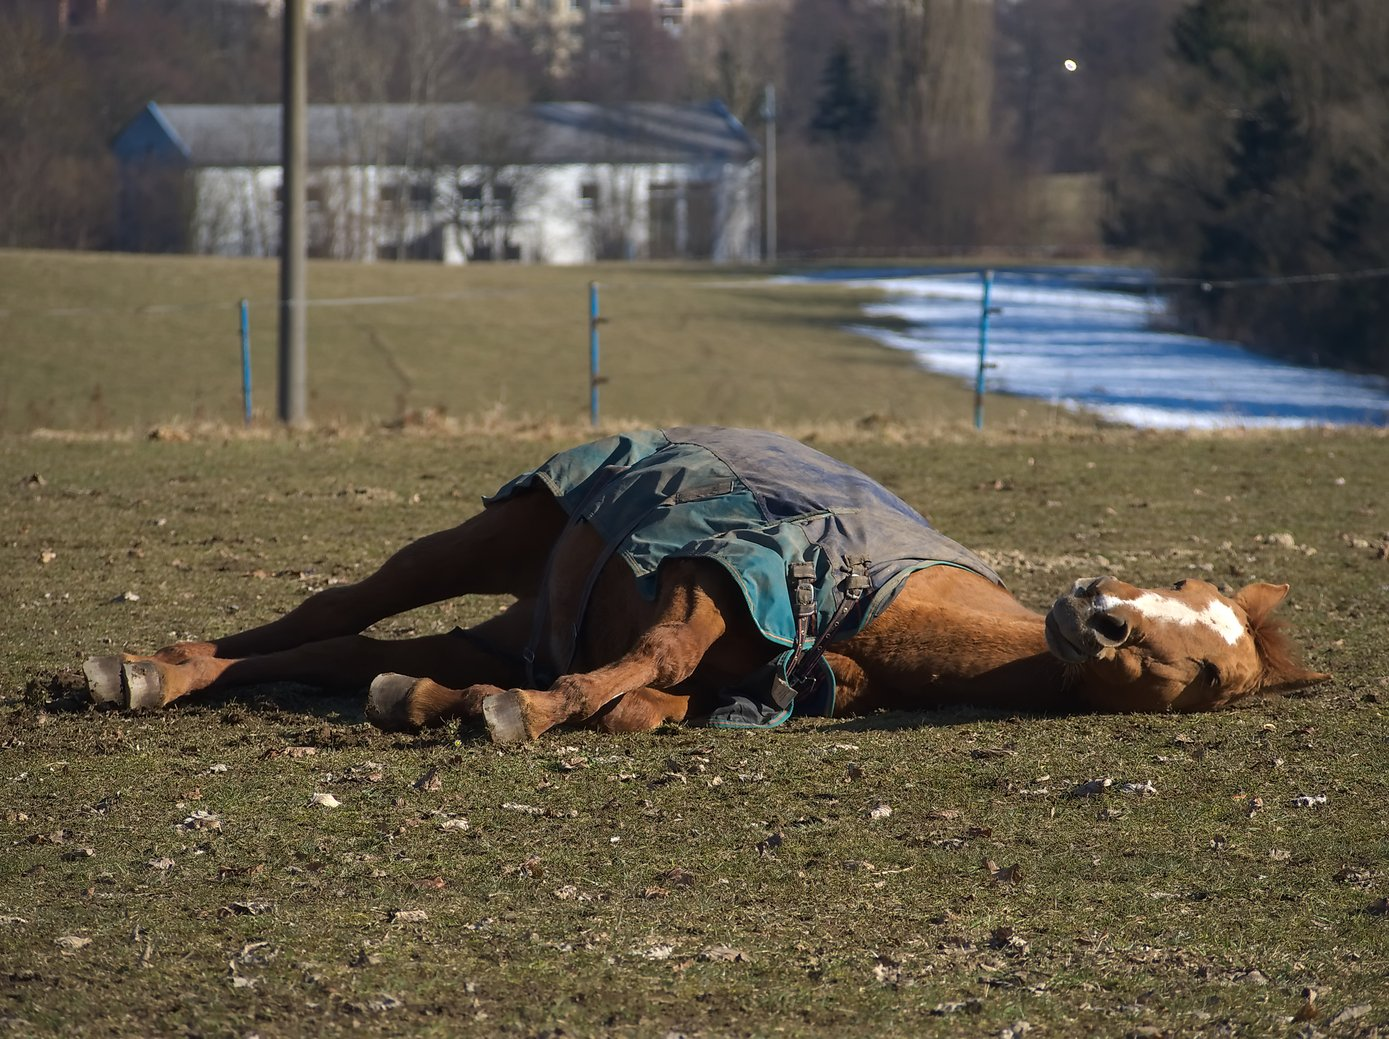
\includegraphics[width=1.0\textwidth]{horse_original.jpg}
        \caption{Původní obrázek.}
    \end{subfigure}
    \hspace{1cm}
    \begin{subfigure}[t]{0.25\textwidth}
        \vskip 0pt
        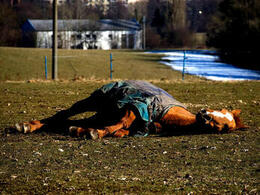
\includegraphics[width=1.0\textwidth]{horse_contrast_plus.jpg}
        \caption{Zvýšený o~50\%}
    \end{subfigure}
    \caption{Výsledky operace úpravy kontrastu}
    \label{fig:contrast}
\end{figure}


\subsubsection{Rozmazání}
Efekt rozmazání se docílí pomocí zprůměrování hodnot současného okolních pixelů.
Současná implementace je v~tomto případě záležitostí použité knihovny \texttt{image}.

\subsubsection{Rotace odstínu}
Tato operace pracuje s~HSV nebo HSL barevným prostorem \cite{wiki:HSL_and_HSV}.
Každý pixel obrázku se převede do odpovídající HSL / HSV reprezentace a~upraví se hodnota H~(hue).
Tato hodnota udává velikost úhlu otočení kolem osy barevného válce, je tedy periodická a~nabývá hodnoty 0~až $360^\circ$.
Hodnoty podle úhlu jsou znázorněny na obrázku \ref{fig:huerotate-scale}.
\begin{figure}[h]
    \centering
    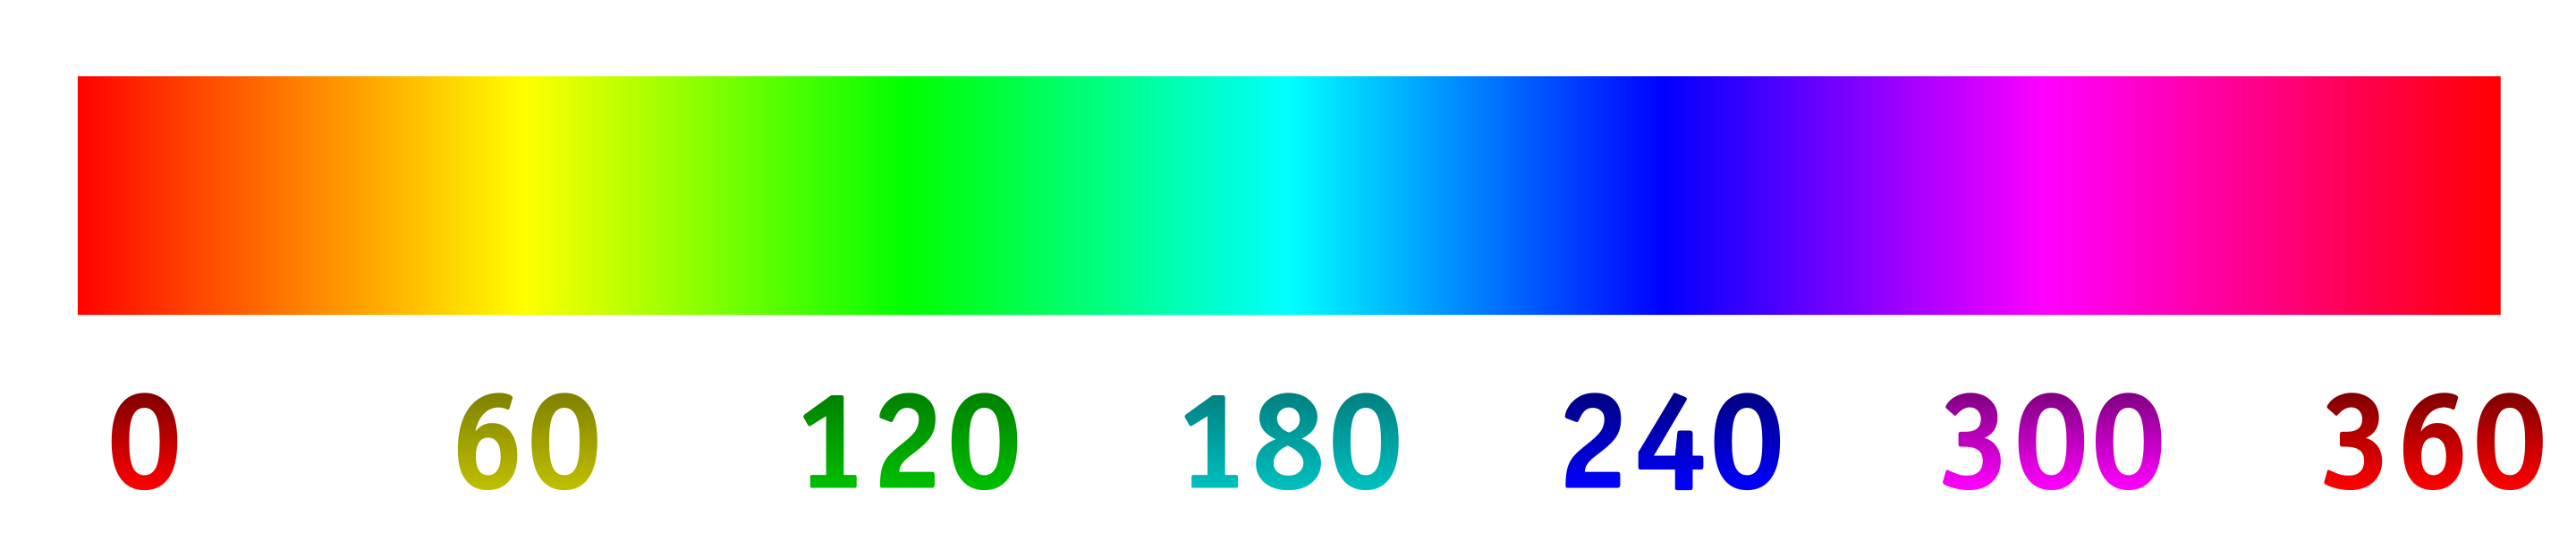
\includegraphics[width=7cm]{hue_scale.png}
    \caption{Barvy odpovídající úhlu H~v HSV nebo HSL modelu \cite{wiki:Hue}.}
    \label{fig:huerotate-scale}
\end{figure}

Na obrázku \ref{fig:huerotate-res} jsou vidět aplikované inkrementy H~o určitý úhel.
\begin{figure}[h]
    \centering
    \begin{subfigure}[t]{0.4\textwidth}
        \vskip 0pt
        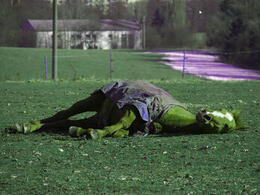
\includegraphics[width=1.0\textwidth]{horse_hue_60.jpg}
        \caption{$H + 60^\circ$}
    \end{subfigure}
    \hspace{1cm}
    \begin{subfigure}[t]{0.4\textwidth}
        \vskip 0pt
        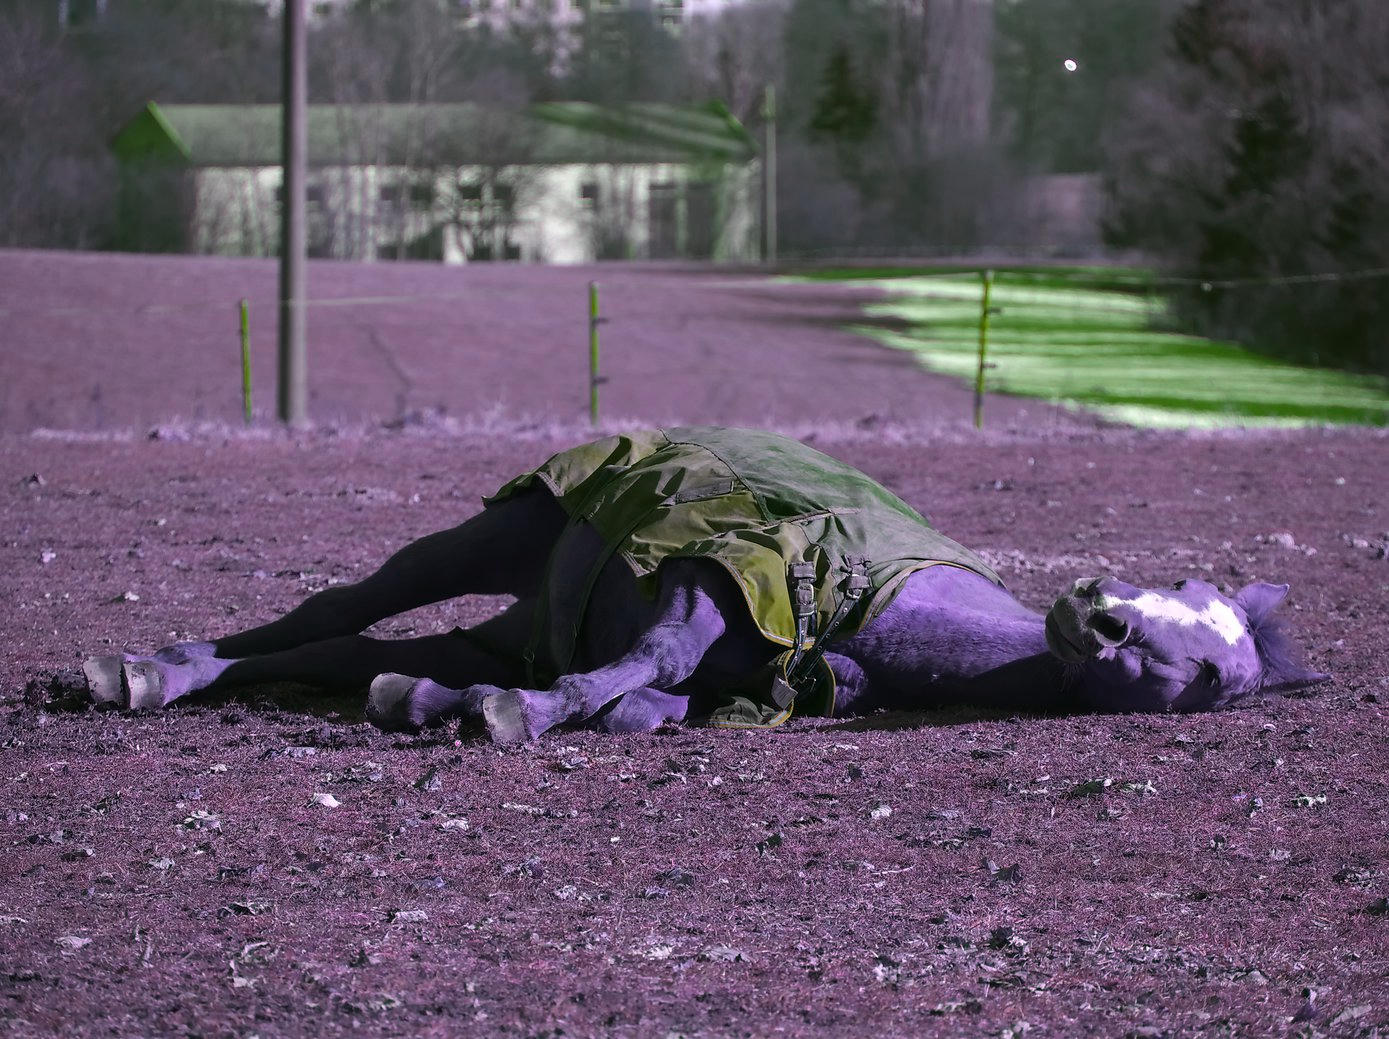
\includegraphics[width=1.0\textwidth]{horse_hue_240.jpg}
        \caption{$H + 240^\circ$}
    \end{subfigure}
    \caption{Ukázka rotace odstínu o~určité úhly.}
    \label{fig:huerotate-res}
\end{figure}

\subsubsection{Vlastní operace zesvětlení}
Jelikož operace \uv{expozice} a~\uv{gamma} nedávají moc pěkné výsledky.
Byla experimentální formou implementována vlastní formule, která se pokouší o~zesvětlení a~ztmavení obrazu při zachování vnímaného kontrastu.
Finální filtr se v~aplikaci jmenuje \uv{Brightness multiply luma}, a~vyhází z~násobení každého pixelu konstantou, které jse pro srovnání implementováno jako filtr \uv{Brightness multiply}.
Uživatel v~editoru nastaví hodnotu $a \in \langle-5,5\rangle$, ze kterého se vypočítá koeficient $c$:
$$c=1+a\,(1 - Y^\gamma)$$
, kde $Y$ je světelná složka z~YUV barevného modelu\cite{wiki:YCbCr} daného pixelu a~$\gamma \in \langle0,1;1,5\rangle$ je rovněž nastavitelná v~GUI a~ve výchozím stavu má hodnotu $0,5$.
Koeficientem $c$ je následně Y~složka vynásobena a~barva pixelu je opět korektně převedena na RGB hodnotu.
Operace má tedy vestavěnou gamma korekci a~světelnost se upravuje pomocí skutečné světelné složky.
Na obrázku \ref{fig:multiplication-luma} je vidět finální výsledek:
\begin{figure}[h]
    \centering
    \begin{subfigure}[t]{0.25\textwidth}
        \vskip 0pt
        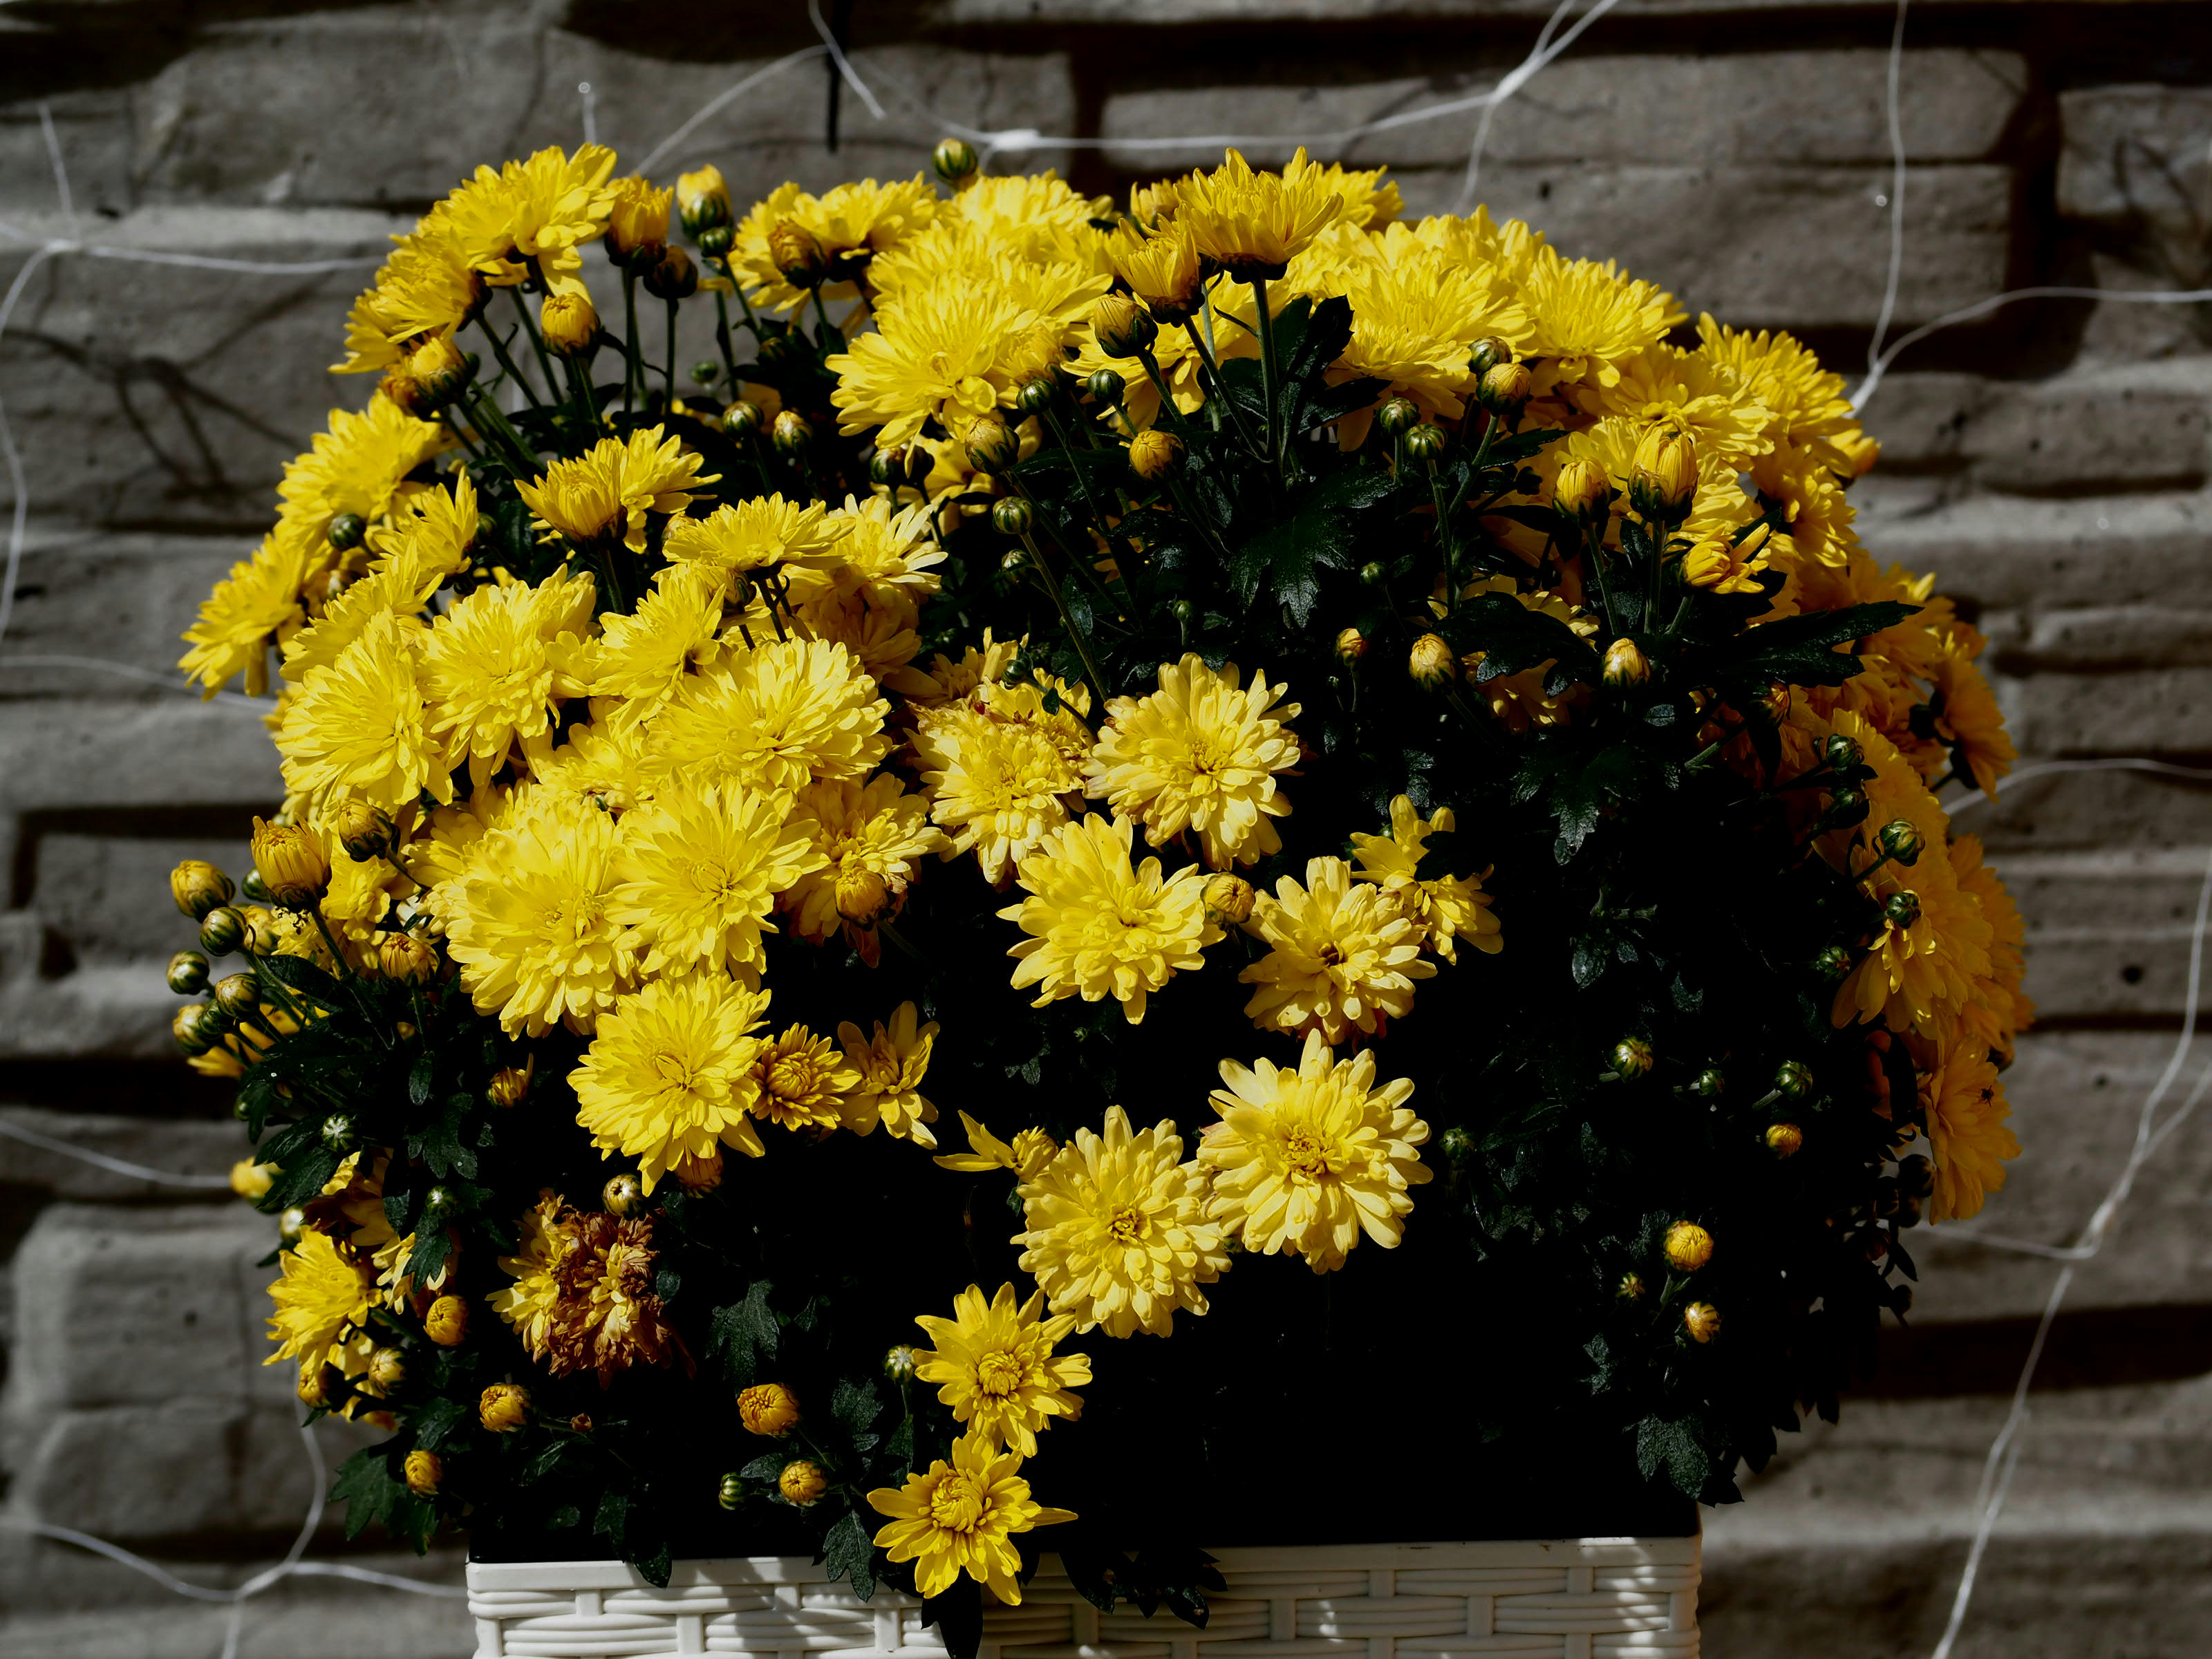
\includegraphics[width=1.0\textwidth]{kvetina_mul_down.jpg}
        \caption{$a = -2$ -- tmavší}
    \end{subfigure}
    \hspace{1cm}
    \begin{subfigure}[t]{0.25\textwidth}
        \vskip 0pt
        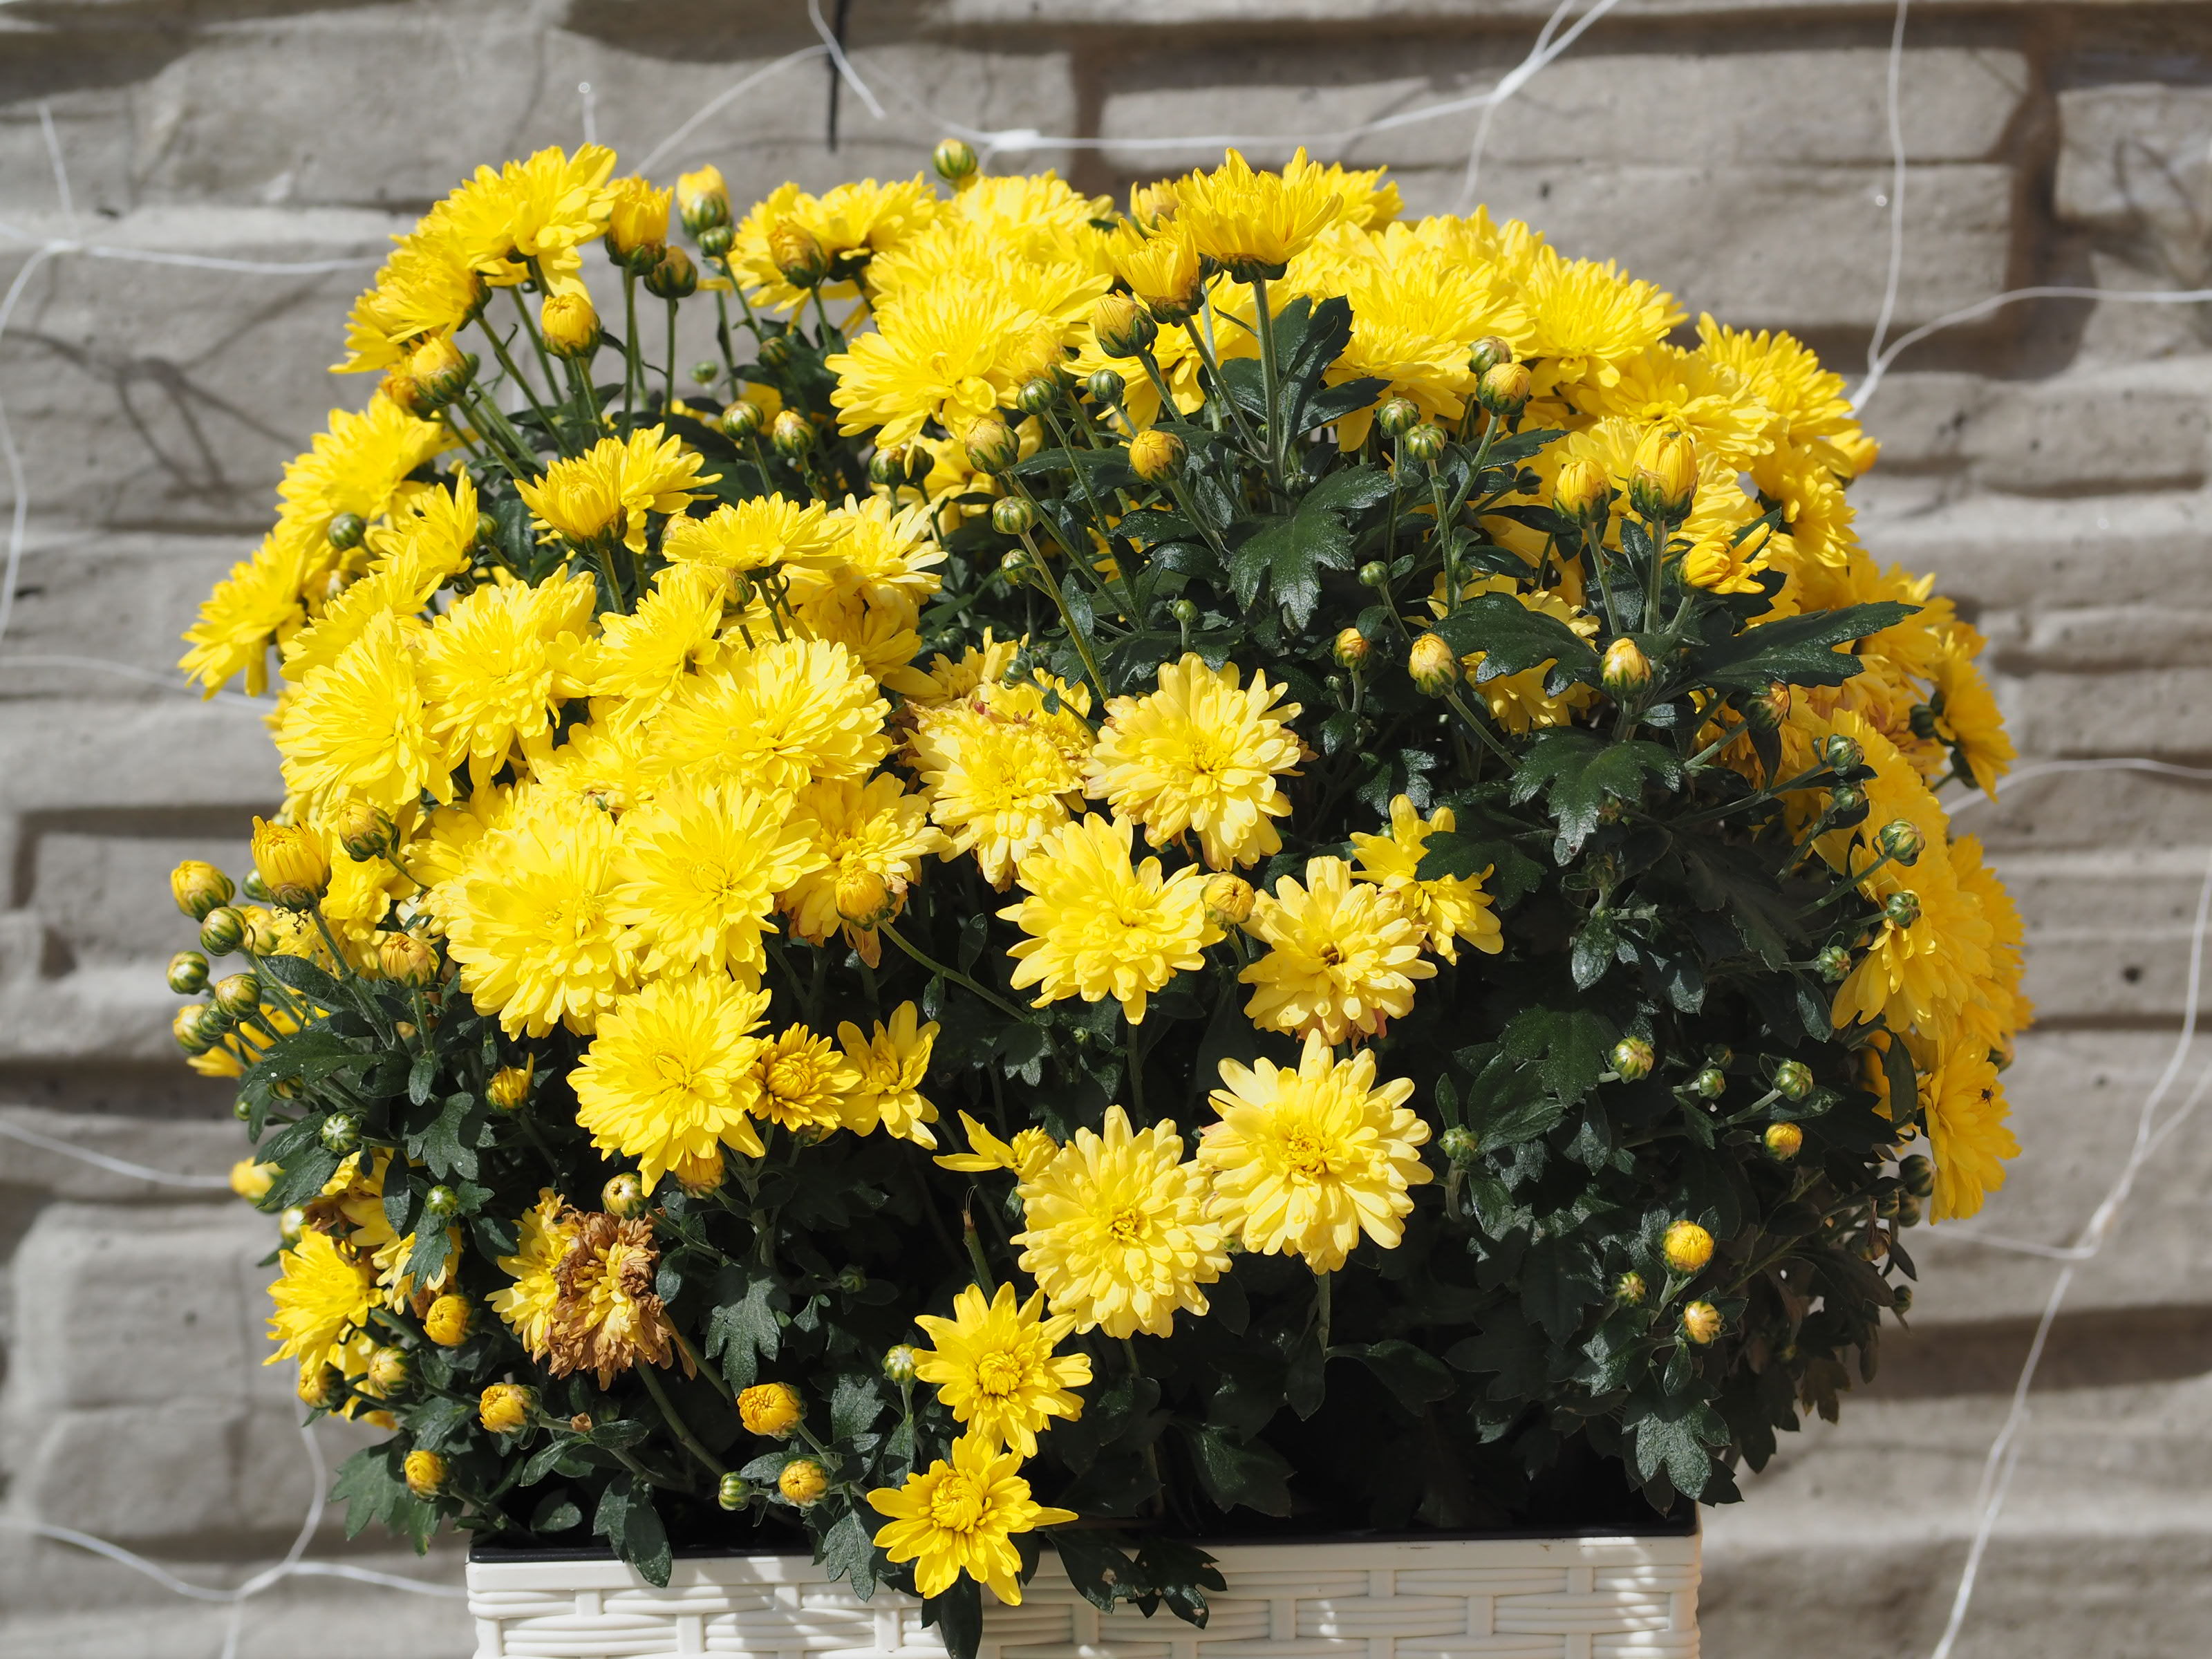
\includegraphics[width=1.0\textwidth]{kvetina.jpg}
        \caption{$a = 0$ -- původní}
    \end{subfigure}
    \hspace{1cm}
    \begin{subfigure}[t]{0.25\textwidth}
        \vskip 0pt
        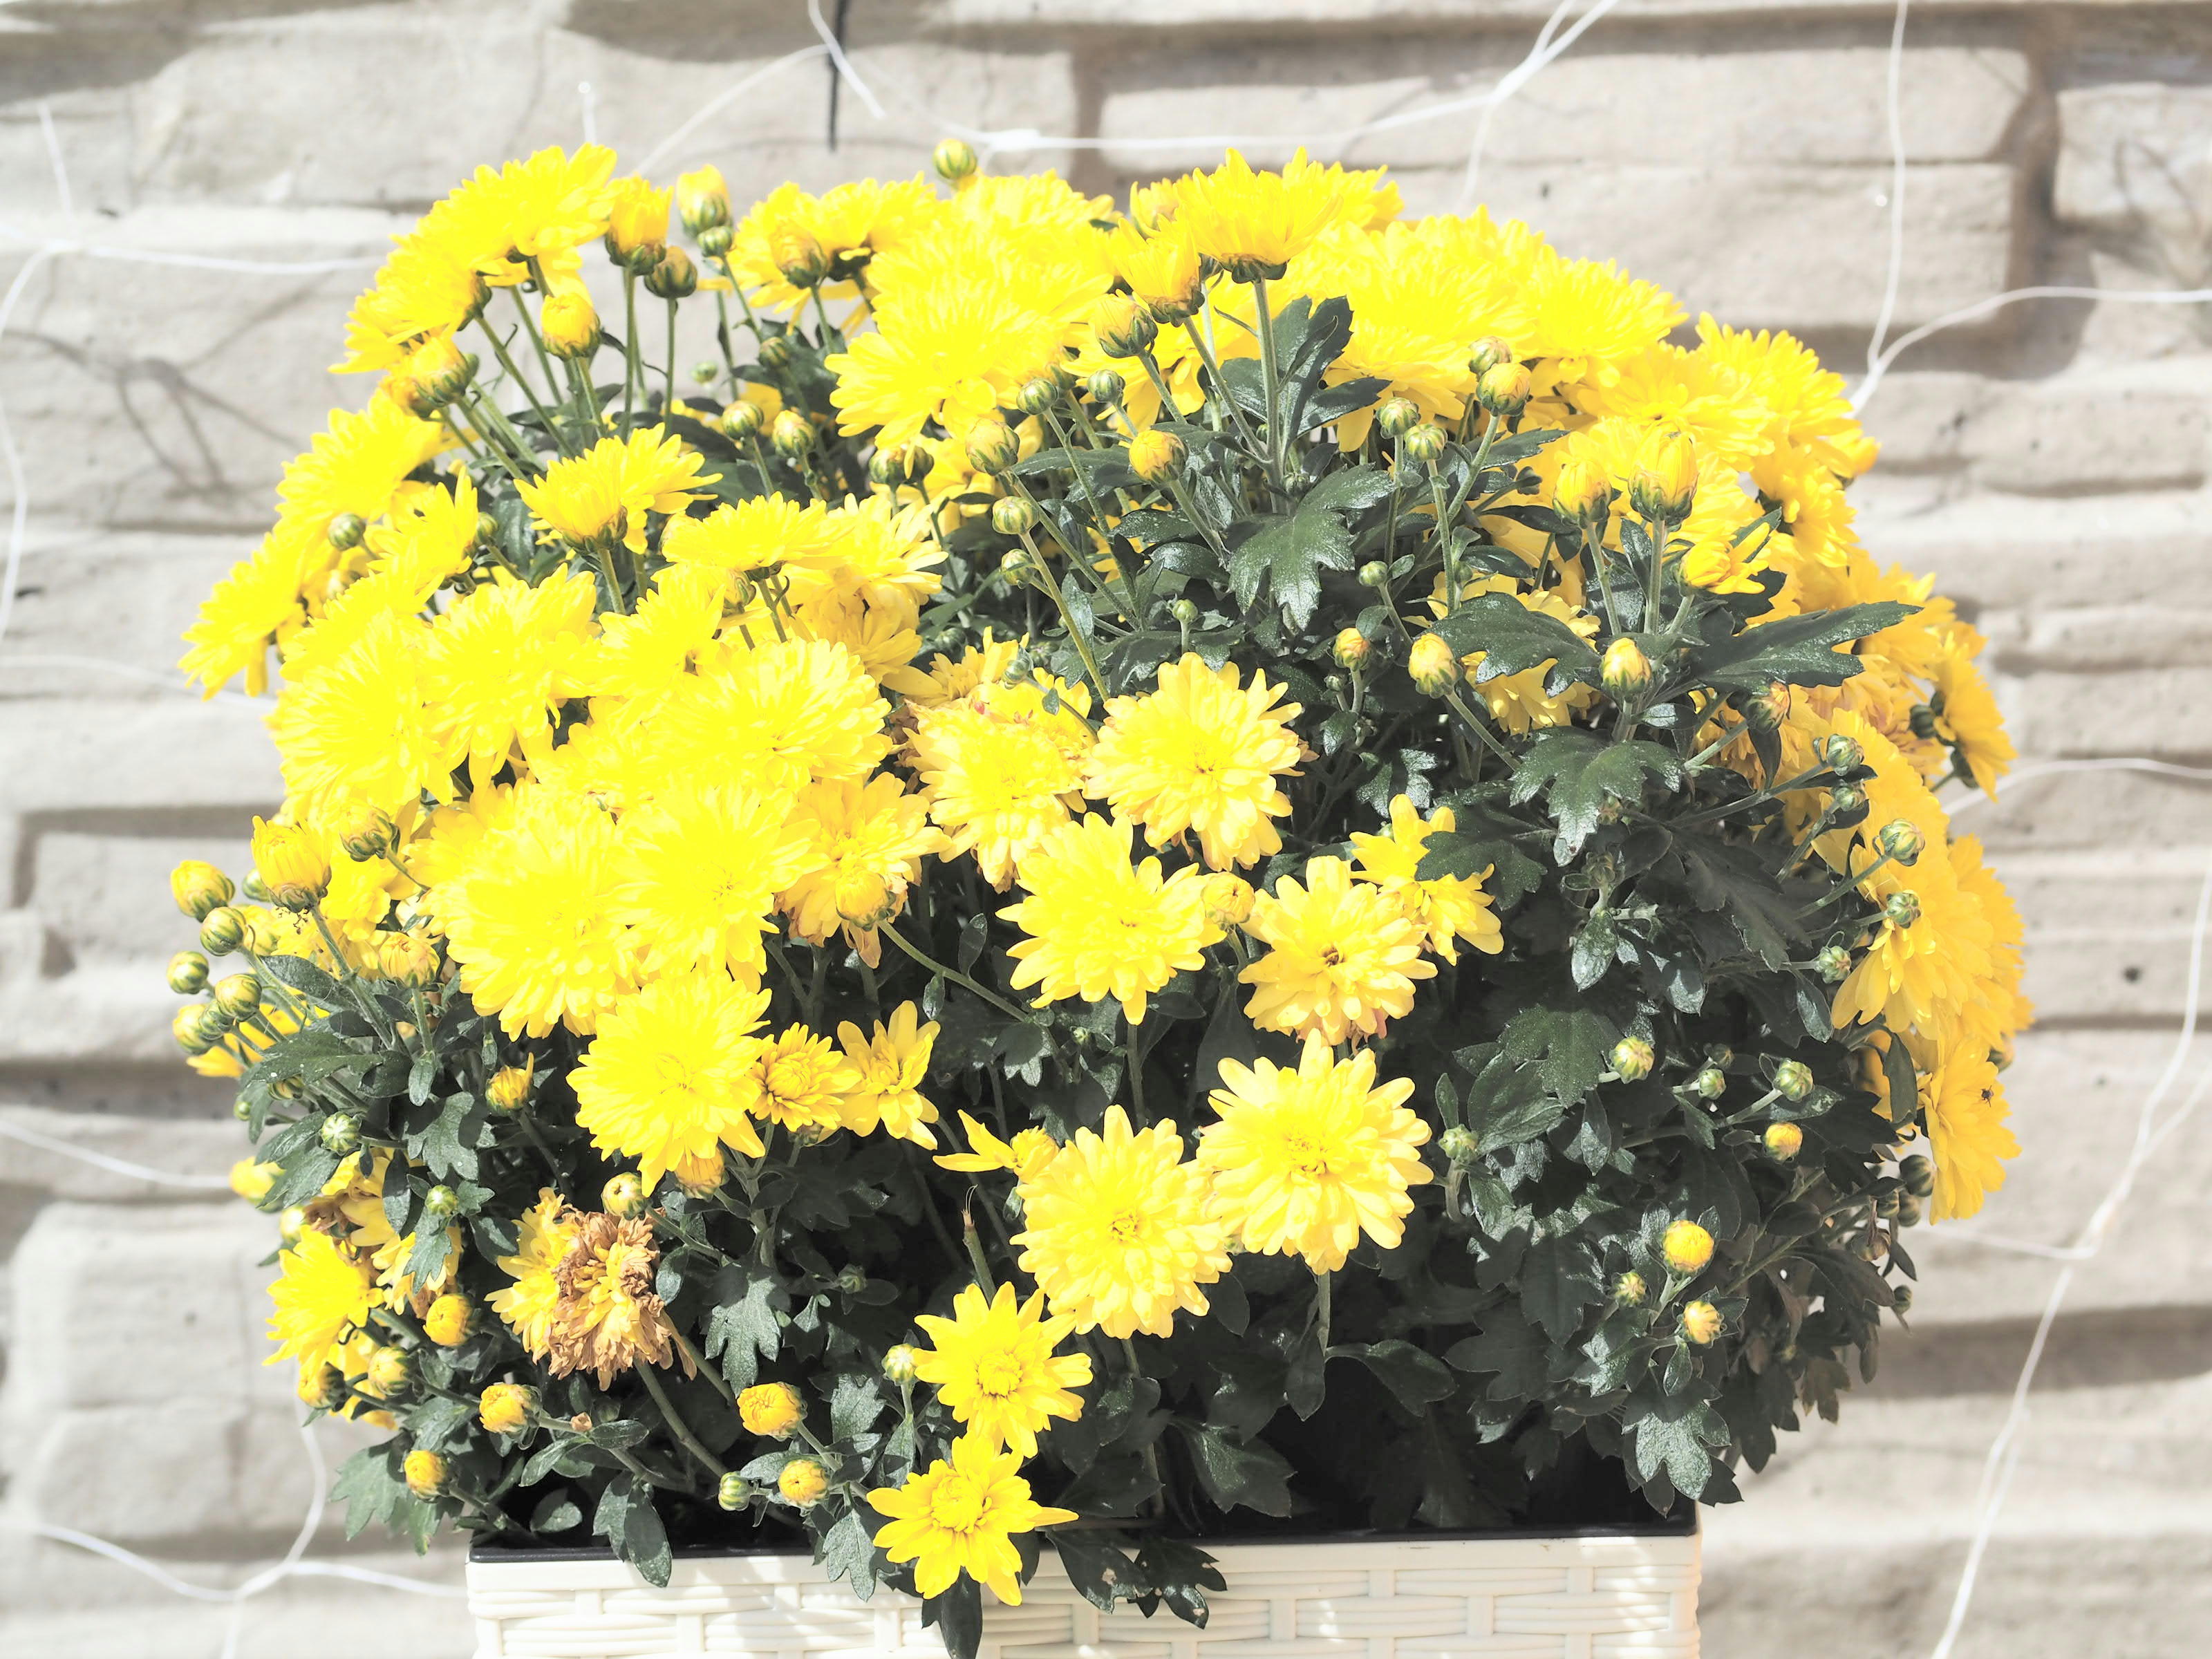
\includegraphics[width=1.0\textwidth]{kvetina_mul_up.jpg}
        \caption{$a = 2$ -- světlejší}
    \end{subfigure}
    \caption{Ztmavení a~zesvětlení pomocí vlastní formule.}
    \label{fig:multiplication-luma}
\end{figure}

\subsection{Obecné barevné transformace a~vlastní filtry}
Aplikace umožňuje nadefinovat vlastní transformaci barev:
$$
P'
=
\begin{bmatrix}
    A_r & A_g & A_b \\
    B_r & B_g & B_b \\
    C_r & C_g & C_b \\
\end{bmatrix}
\cdot
\begin{bmatrix}R\\G\\B\end{bmatrix}
$$
Kde $A_x$, $B_x$ a~$C_x$ si lze libovolně navolit v~intervalu $\langle0, 2\rangle$.
Díky tomuto lze například implementovat vlastní filtry.
Vísledek lze vidět na obrázku \ref{fig:custom-filters}.
\begin{figure}[h]
    \centering
    \begin{subfigure}[t]{0.3\textwidth}
        \centering
        \vskip 0pt
        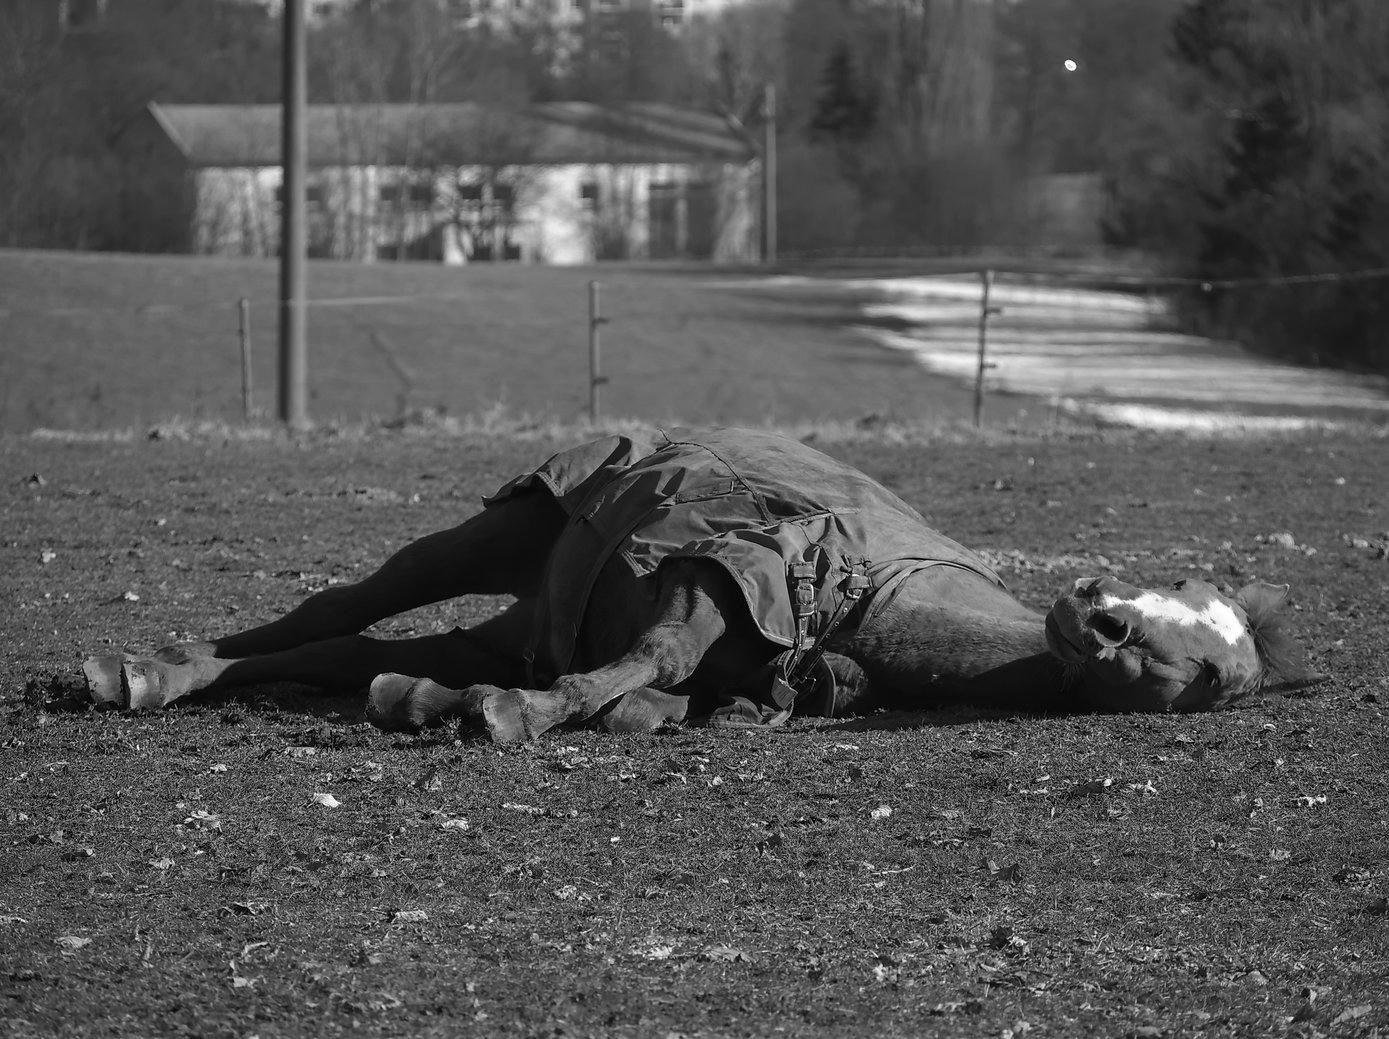
\includegraphics[width=0.8\textwidth]{horse_average.jpg}
        \caption{
        $
            \begin{bmatrix}
                1/3 & 1/3 & 1/3 \\
                1/3 & 1/3 & 1/3 \\
                1/3 & 1/3 & 1/3 \\
            \end{bmatrix}
            \cdot
            \begin{bmatrix}R\\G\\B\end{bmatrix}
        $\\\\Luma nekorektní černobílá
        }
    \end{subfigure}
    \hspace{0.1cm}
    \begin{subfigure}[t]{0.3\textwidth}
        \centering
        \vskip 0pt
        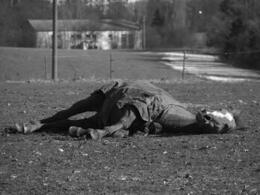
\includegraphics[width=0.8\textwidth]{horse_luma.jpg}
        \caption{
            $
            \begin{bmatrix}
                0,299 & 0,587 & 0,114 \\
                0,299 & 0,587 & 0,114 \\
                0,299 & 0,587 & 0,114 \\
            \end{bmatrix}
            \cdot
            \begin{bmatrix}R\\G\\B\end{bmatrix}
            $\\\\Luma korektní černobílá
        }
    \end{subfigure}
    \hspace{0.1cm}
    \begin{subfigure}[t]{0.3\textwidth}
        \centering
        \vskip 0pt
        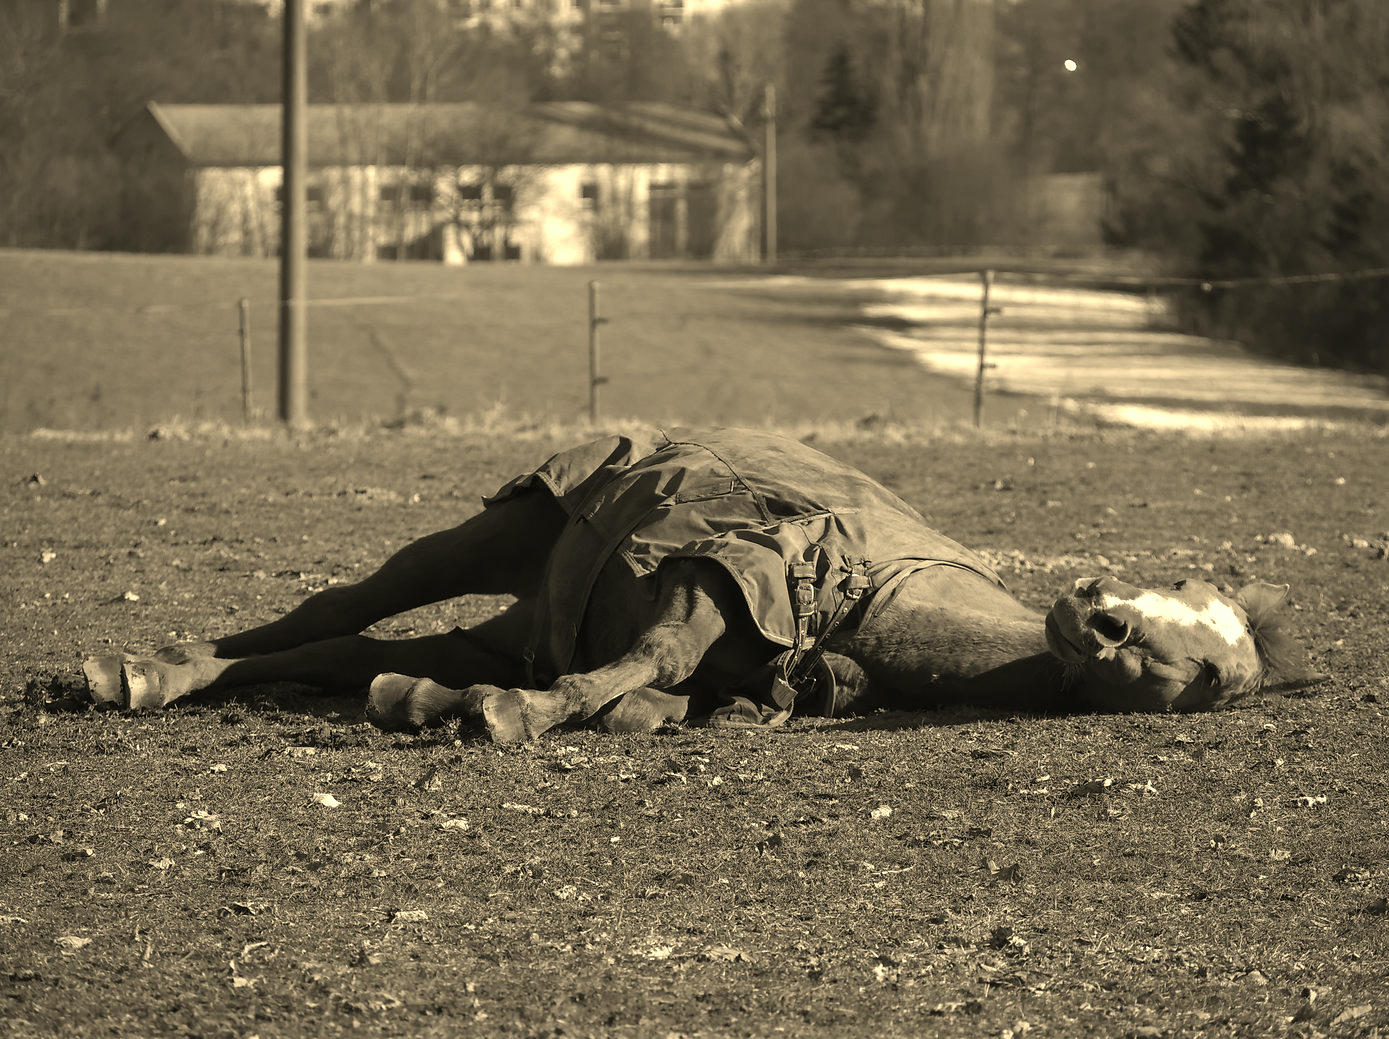
\includegraphics[width=0.8\textwidth]{horse_sepia.jpg}
        \caption{
            $
            \begin{bmatrix}
                0,393 & 0,769 & 0,189 \\
                0,349 & 0,686 & 0,168 \\
                0,272 & 0,534 & 0,131 \\
            \end{bmatrix}
            \cdot
            \begin{bmatrix}R\\G\\B\end{bmatrix}
            $\\\\Efekt \uv{sépie}\cite{Howtocon48:online}
        }
    \end{subfigure}
    \caption{Demonstrace příkladů vlastních filtrů.}
    \label{fig:custom-filters}
\end{figure}
Filtru lze také nastavit mírů aplikování, tedy lineární interpolaci mezi původním obrázkem a~plně transformovaným.

\subsection{Ostatní implementační detaily}
\subsubsection{škálování náhledu}
Aplikace pracuje s~daty obrázku v~nekomprimovaném stavu, to znamená, že větší fotky mohou zabírat desítky megabajtů, aplikace proto provádí veškeré operace nad zmenšenou verzí původního obrazu podle velikosti náhledu na obrazovce uživatele.
V dolní liště je vidět, jako poslední údaj, rozlišení obrázku, který se používá pro živý náhled a~na FullHD (1920x1080) monitoru tato velikost nepřesahuje 4MB.
Filtry jsou aplikovány na obrázek v~plném rozlišení pouze jednou a~to při jeho uložení do souboru.

\section{Závěr}
Aplikace je jednoduchý aplikátor filtrů na obrázky s~možností jejich ukládání a~živého náhledu.
Je uživatelsky jednoduchá a~nabízí nástroje, které umožní uživateli pochopit principy obrazových barevných filtrů na nejnižší úrovni. Z časových důvodu bohužel nebyla implementována možnost ořezání ani změna velikosti obrázku ani možnost spouštět a editovat videosekvence.

Repozitář aplikace je dostupný veřejně online na platformě GitHub\footnote{\url{https://github.com/xfusek08/mul-image-edit-rs}} a~k jejímu sestavení je třeba mít nainstalovaný balíčkovací systém \texttt{cargo}\footnote{\url{https://www.rust-lang.org/tools/install}}.

\bibliographystyle{alpha}
\begin{flushleft}
  \bibliography{project}
\end{flushleft}

%\appendix
%\newpage
%\section{}

\end{document}
